\documentclass[10pt,a4paper]{article}
\usepackage[T1]{fontenc}
\usepackage[utf8]{inputenc}
\usepackage{graphicx}
\usepackage{parskip}
\usepackage{subcaption}
\usepackage{tabularx}
\usepackage{hyperref}
\usepackage[a4paper,margin=1in]{geometry}
\usepackage[polish]{babel}
\usepackage{float}

\title{Aplikacja EntertainMatch -- Raport końcowy}
\author{Adrian Bednarz, Bartłomiej Dach}

\begin{document}

\maketitle

\section{Opis aplikacji}

Aplikacja EntertainMatch przeznaczona jest dla wieloosobowych grup znajomych.
Za jej pomocą użytkownicy z grupy wspólnie wybierają wydarzenie, na które chcą się wybrać,
przechodząc przez wieloetapowy proces głosowania, złożony z:

\begin{itemize}
	\item wyboru kategorii wydarzenia (np. filmy, koncerty),
	\item wyboru konkretnego wydarzenia z danej kategorii (wydarzenia są wybierane ręcznie przez
		deweloperów w obrębie poszczególnych miast). Użytkownicy mogą przejrzeć wybrane
		informacje o wydarzeniach, zależne od kategorii (np. w przypadku filmów są to:
		zwiastun filmu, krótki opis, obsada, reżyser, czas trwania i ocena filmu wg agregatora
		recenzji Rotten Tomatoes);
	\item wyboru miejsca oraz daty dla danego wydarzenia (możliwe jest wyświetlenie za pomocą
		aplikacji Google Maps dokładnej lokalizacji),
	\item deklaracji, czy dany użytkownik może przyjść na dane wydarzenie w danym terminie.
\end{itemize}

Poszczególni użytkownicy nie znają wyborów podjętych przez innych w obrębie głosowania, aby nie
sugerować się ich wyborami.
W przypadku remisu w obrębie danego etapu, głosowanie jest zawężane do najczęściej wybieranych
do tej pory; w przypadku kolejnego remisu wynik wybierany jest losowo.
Każda zmiana etapu powoduje wyświetlenie powiadomień u wszystkich użytkowników.

Po zakończeniu głosowania, wydarzenia są dodawane do odpowiedniej zakładki w głównym widoku.
Dodatkowo, jeśli użytkownik zezwoli aplikacji na dostęp do terminarza, dodawane jest do niego
przypomnienie na dzień, w którym dane wydarzenie ma się odbyć. Wydarzenia usuwane są z listy po
zakończeniu.

\begin{figure}
	\centering
	\begin{subfigure}[t]{0.4\textwidth}
		\centering
		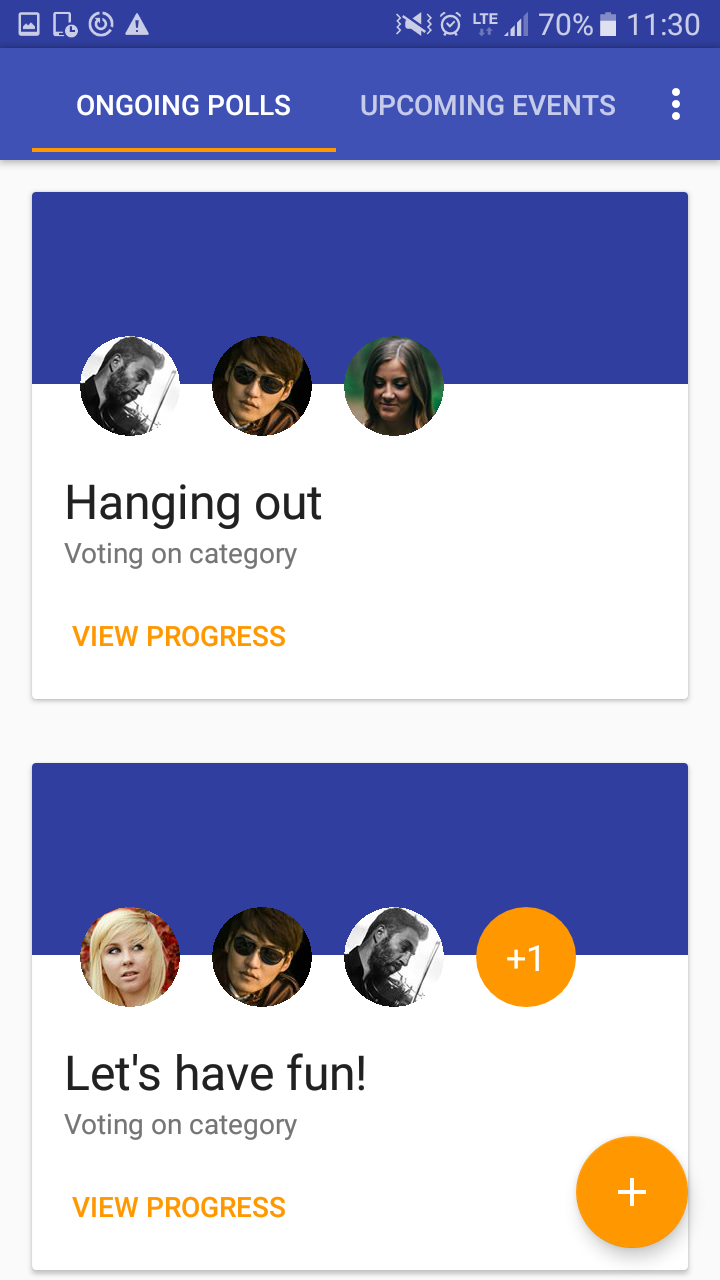
\includegraphics[width=0.9\textwidth]{screen1.png}
		\caption{Główny widok aplikacji, zawierający toczące się głosowania oraz nadchodzące
		wydarzenia}
	\end{subfigure}
	\hfill
	\begin{subfigure}[t]{0.4\textwidth}
		\centering
		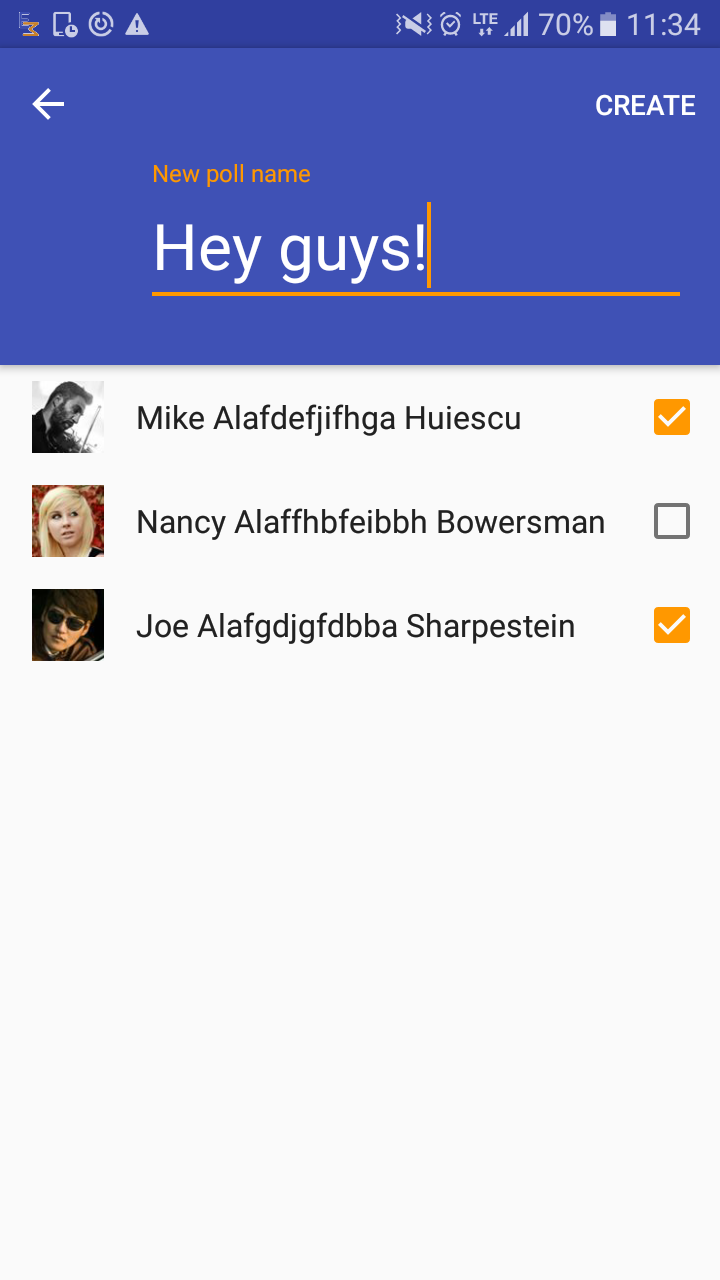
\includegraphics[width=0.9\textwidth]{screen2.png}
		\caption{Ekran dodawania nowego głosowania}
	\end{subfigure}

	\begin{subfigure}[t]{0.4\textwidth}
		\centering
		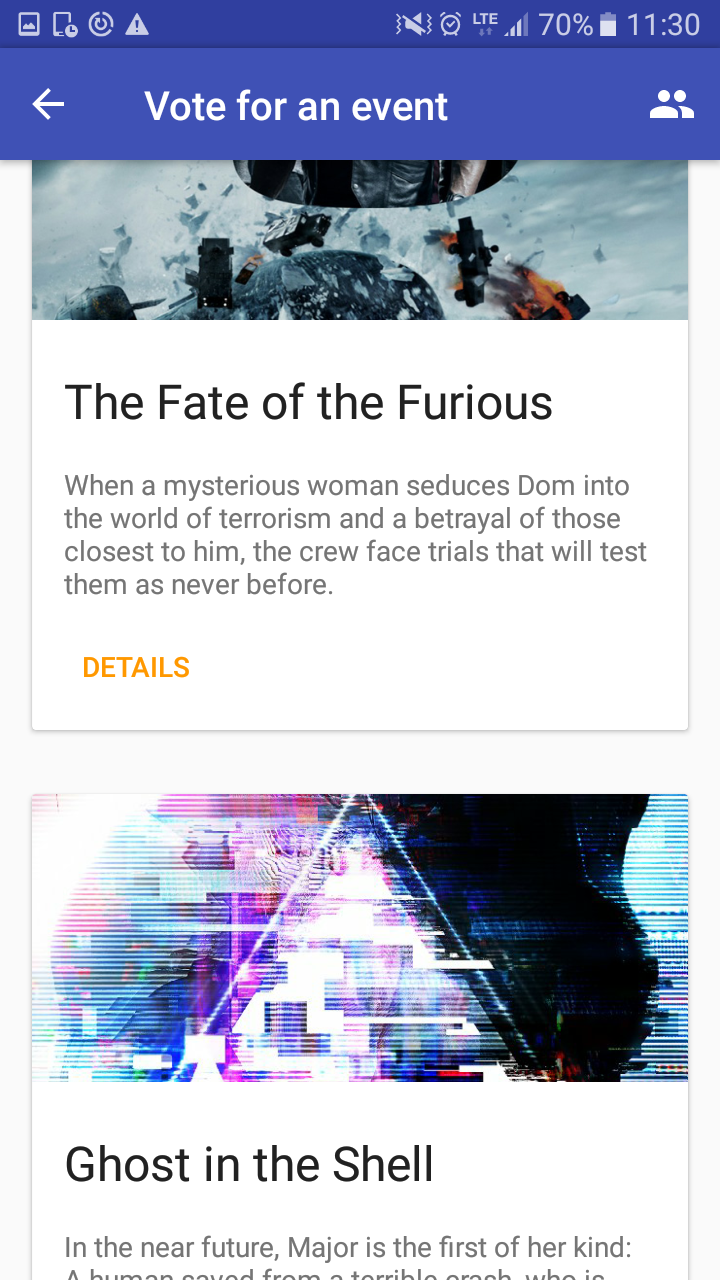
\includegraphics[width=0.9\textwidth]{screen3.png}
		\caption{Głosowanie na etapie wyboru wydarzenia}
	\end{subfigure}
	\hfill
	\begin{subfigure}[t]{0.4\textwidth}
		\centering
		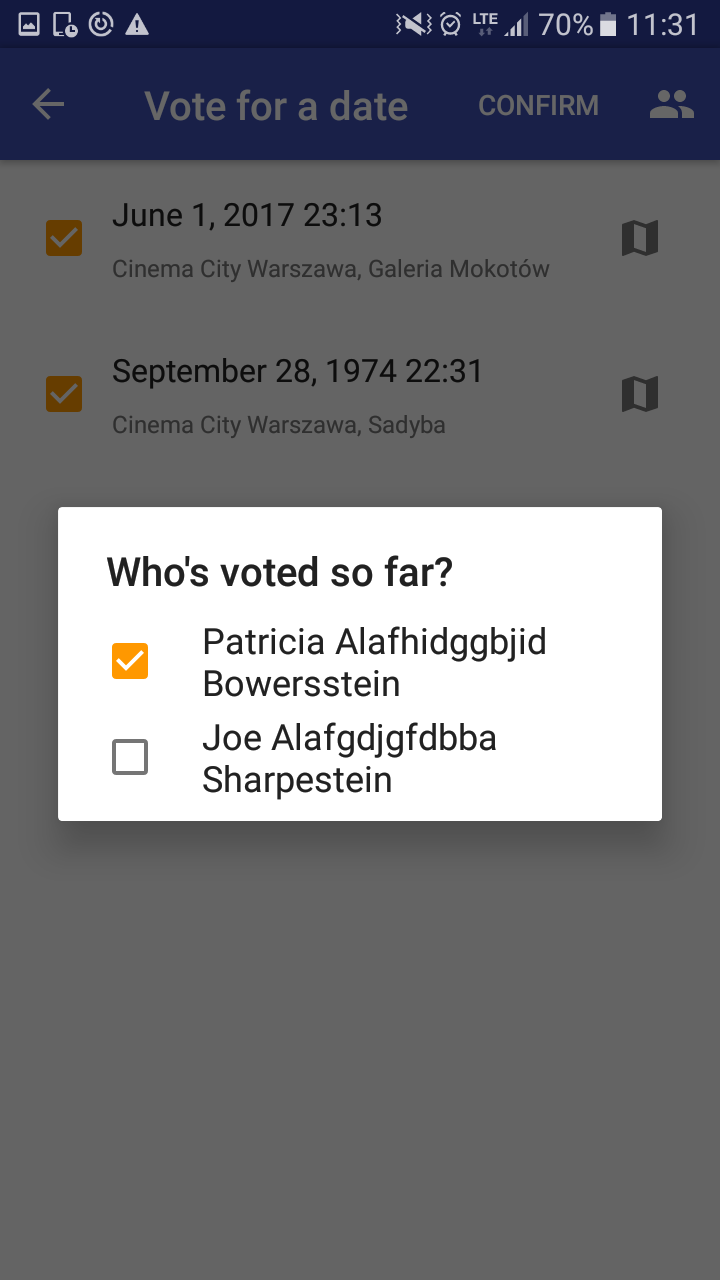
\includegraphics[width=0.9\textwidth]{screen4.png}
		\caption{Głosowanie na etapie wyboru daty. Widoczne są opcje: podglądu danej lokalizacji
		dla wydarzenia oraz sprawdzenia, który z użytkowników zagłosował już w danym etapie}
	\end{subfigure}
	\caption{Przykładowe widoki interfejsu użytkownika aplikacji}
\end{figure}

%\section{Logika biznesowa}

\section{Wykorzystane narzędzia i wzorce projektowe}

W aplikacji wykorzystywana jest baza danych dostarczana przez usługę Firebase \cite{firebase},
dostarczająca asynchroniczne aktualizacje danych do aplikacji, gdy aplikacja jest połączona
z Internetem za pośrednictwem usług Google Play.
Aktualizacje te obsługiwane są w aplikacji za pomocą pakietu Reactive Extensions oraz mechanizmu
tzw. obiektów obserwowalnych (ang. \texttt{Observable}).
Obiekty te reprezentują strumień asynchronicznych zdarzeń, na które można reagować, dodając
do obserwowalnego obiektu subskrypcję.

Logowanie do aplikacji odbywa się za pośrednictwem Facebook SDK \cite{facebook-sdk}.
W aplikacji do głosowań można dodawać znajomych z Facebooka, którzy zainstalowali aplikację.

Część komponentów aplikacji implementuje wzorzec wstrzykiwania zależności i inwersji kontroli.
W celu wstrzykiwania użyty został kontener Dagger \cite{dagger}.
Pozwala on na lepsze odseparowanie funkcjonalności, poprawia możliwości testowania oraz wspiera
kompozycję klas.

Przy projektowaniu i implementacji interfejsu użytkownika użyto biblioteki Butter Knife
\cite{butterknife}, która pozwala wiązać pola w klasach aktywności z widokami definiowanymi
w kodzie XML.
Dodatkowo w celu wyświetlania obrazów z Internetu, wykorzystana została biblioteka Picasso
\cite{picasso}, zapewniająca dynamiczne ładowanie obrazów oraz ich \emph{caching} na dysku.

W celu ułatwienia pisania kodu, użyta została biblioteka Lombok \cite{lombok}, pozwalająca
na automatyczne generowanie getterów, setterów i konstruktorów.

W przykładowych testach wykorzystany został framework do testowania JUnit \cite{junit},
biblioteka Mockito \cite{mockito} do tworzenia tzw. mocków oraz AssertJ \cite{assertj} wspomagająca
pisanie asercji w testach jednostkowych.
Dodatkowo dołączone zostało kilka testów interfejsu, używających biblioteki Espresso \cite{espresso}
w celu automatyzowanego wykonywania kliknięć.

\section{Raport z testów z użytkownikami}

Poniżej znajduje się lista testów z użytkownikami wykonanych w trakcie tworzenia aplikacji. Większość
z uwag została uwzględniona i poprawiona w ostatecznej wersji.

\begin{enumerate}
	\item Zalogowanie się do aplikacji
		\begin{itemize}
			\item \textbf{Opis testu:}
				Użytkownik po zainstalowaniu aplikacji loguje się za pośrednictwem
				konta w serwisie Facebook.
			\item \textbf{Przewidywany rezultat:}
				Po poprawnym zalogowaniu się następuje przejście do głównego ekranu
				aplikacji.
			\item \textbf{Wynik testu:} Pozytywny
			\item \textbf{Uwagi:} Brak.
		\end{itemize}
	\item Dodanie nowego głosowania
		\begin{itemize}
			\item \textbf{Opis testu:}
				Użytkownik z poziomu głównego ekranu przechodzi do widoku dodawania
				nowego głosowania, wypełnia go i zatwierdza wprowadzone dane.
			\item \textbf{Przewidywany rezultat:}
				W głównym ekranie aplikacji pojawia się dodane głosowanie.
			\item \textbf{Wynik testu:} Pozytywny
			\item \textbf{Uwagi:}
				Myląca ikona na przycisku dodającym głosowania, dodane głosowania
				pojawiały się na końcu listy, brak domyślnej nazwy głosowania.
		\end{itemize}
	\item Głosowanie na kategorię
		\begin{itemize}
			\item \textbf{Opis testu:}
				Użytkownik w głównym ekranie wybiera głosowanie znajdujące się na
				etapie kategorii i oddaje głos na jedną z nich.
			\item \textbf{Przewidywany rezultat:}
				Głos zostaje zarejestrowany; jeśli głosujący był ostatni, następuje
				przejście do kolejnego etapu.
			\item \textbf{Wynik testu:} Pozytywny
			\item \textbf{Uwagi:}
				Kliknięcie na obrazek reprezentujący kategorię nie powoduje reakcji,
				brak możliwości podejrzenia głosów innych użytkowników lub sprawdzenia
				kto zagłosował w danym etapie.
		\end{itemize}
	\item Głosowanie na wydarzenie
		\begin{itemize}
			\item \textbf{Opis testu:}
				Użytkownik w głównym ekranie wybiera głosowanie znajdujące się na
				etapie wydarzeń i oddaje głos na jedno z nich.
			\item \textbf{Przewidywany rezultat:} 
				Rejestracja głosu, przejście do kolejnego etapu.
			\item \textbf{Wynik testu:} Pozytywny
			\item \textbf{Uwagi:}
				Snackbar informujący o sposobie głosowania niepotrzebnie pojawiał się
				za każdym razem.
		\end{itemize}
	\item Głosowanie na datę
		\begin{itemize}
			\item \textbf{Opis testu:}
				Użytkownik w głównym ekranie wybiera głosowanie znajdujące się na
				etapie daty i oddaje głos na jedno z nich.
			\item \textbf{Przewidywany rezultat:} 
				Rejestracja głosu, przejście do kolejnego etapu.
			\item \textbf{Wynik testu:} Pozytywny
			\item \textbf{Uwagi:} Brak.
		\end{itemize}
	\item Potwierdzenie lub odmowa potwierdzenia obecności
		\begin{itemize}
			\item \textbf{Opis testu:}
				Użytkownik wybiera w głównym ekranie zakończone głosowanie i potwierdza
				lub odmawia potwierdzenia obecności w wybranym terminie.
			\item \textbf{Przewidywany rezultat:} 
				Wybór użytkownika zostaje zapisany, głosowanie znika z listy. W przypadku
				zgody w zakładce z wydarzeniami dodane jest nowe wydarzenie; dodatkowo,
				jeśli użytkownik wyrazi zgodę, dodawane jest również w terminarzu
				przypomnienie związane z terminem wydarzenia.
			\item \textbf{Wynik testu:} Pozytywny
			\item \textbf{Uwagi:} Brak.
		\end{itemize}
\end{enumerate}

\begin{thebibliography}{99}

	\bibitem{assertj}
		AssertJ,
		Joel Costigliola,
		\url{https://joel-costigliola.github.io/assertj/},
		Apache 2.0

	\bibitem{butterknife}
		Butter Knife,
		Jake Wharton,
		\url{https://jakewharton.github.io/butterknife/},
		Apache 2.0

	\bibitem{dagger}
		Dagger,
		Square,
		\url{https://square.github.io/dagger/},
		Apache 2.0

	\bibitem{espresso}
		Espresso,
		Android Testing Support Library,
		\url{https://google.github.io/android-testing-support-library/docs/espresso/},
		CC BY-SA 2.5

	\bibitem{facebook-sdk}
		Facebook SDK for Android v4.x,
		Facebook for Developers,
		\url{https://developers.facebook.com/docs/android/downloads}

	\bibitem{firebase}
		Firebase,
		Google,
		\url{https://firebase.google.com/}

	\bibitem{junit}
		JUnit,
		\url{http://junit.org/junit4/},
		Eclipse Public License 1.0

	\bibitem{mockito}
		Mockito,
		\url{http://site.mockito.org/},
		MIT

	\bibitem{picasso}
		Picasso,
		Square,
		\url{https://square.github.io/picasso/},
		Apache 2.0

	\bibitem{lombok}
		Project Lombok,
		\url{https://projectlombok.org/},
		MIT

\end{thebibliography}

\end{document}
